\documentclass[final]{beamer}

% Set the dimensions of the poster
\usepackage[orientation=landscape,size=a2,scale=1.5,debug]{beamerposter}  % e.g. custom size poster
\title[R\&P peace]{New evidence violent conflicts between Rabbit-skinners and Poppy-chewers}

\author[Pants]{Fancy Pants}
\date{April 2023}

\definecolor{redcaa}{RGB}{152,0,34}

% Set the font sizes for the headings and text
%\setbeamerfont{title}{size=\Huge}
%\setbeamerfont{author}{size=\huge}
\setbeamerfont{institute}{size=\large}
%\setbeamerfont{block title}{size=\Large}
%\setbeamerfont{block body}{size=\large}


% Remove the navigation symbols at the bottom of the poster
\setbeamertemplate{navigation symbols}{}

% Set the background color of the poster
\setbeamercolor{background canvas}{bg=redcaa}
\setbeamercolor{block,sep=2pt}{bg=white}
\setbeamercolor{structure}{bg=redcaa}

\setbeamercolor{block}{fg=black}
\setbeamercolor{title}{bg=white}
\setbeamercolor{block title}{fg=redcaa,bg=white}
\setbeamercolor{block body}{use=block title,bg=block title.bg}
\setbeamercolor{separation line}{fg=redcaa,bg=redcaa}
\setbeamercolor{block separation line}{fg=redcaa,bg=redcaa}
\setbeamercolor{footline}{fg=redcaa,bg=white}
\setbeamercolor{footlinecolor}{bg=white,fg=redcaa}
\setbeamertemplate{blocks}[framed]


\setbeamertemplate{footline}
{ 
    \begin{beamercolorbox}[wd=\paperwidth]{footlinecolor}
        \vskip5pt
        \begin{columns}
            \column{.05\paperwidth}
            \hspace{.2cm}
            
\includegraphics[height=2cm]{caa2023_inv.pdf}
            \column{.75\paperwidth}
            CAA | April 2023 -- 
            \textcolor{redcaa}{\textbf{New evidence violent conflicts between Rabbit-skinners and Poppy-chewers}}
            Fancy Pants
            \column{.05\paperwidth}
            \hfil
        \end{columns}
        \vspace{.1cm}
    \end{beamercolorbox} 
}

% Begin the document
\begin{document}

% Create the title block
\begin{frame}[t]
    \vspace{-.5cm}
    \begin{beamercolorbox}[wd=\paperwidth]{title}
    \vspace{.6cm}
        \begin{columns}

            \column{.15\textwidth}

            \column{.80\textwidth}
            {
                \raggedleft
                \usebeamerfont{title}\textcolor{redcaa}{\textbf{New evidence violent conflicts between Rabbit-skinners and Poppy-chewers}} \par
                \usebeamerfont{author}\textcolor{redcaa}{Fancy Pants}\par
                \usebeamerfont{institute}\textcolor{black}{University Veritas Veritae}\par
            }

            \column{.05\textwidth}
            
\includegraphics[height=3cm]{universHS.png}
        \end{columns}
    \vspace{.8cm}

    \end{beamercolorbox}


    \vspace{2cm}


    \begin{columns}[t]
        %Abstract: This paper presents an analysis of engravings on ceramic artifacts that suggest the presence of conflict between the Poppychewer and Rabbitskinner populations. The engravings depict scenes of violence and aggression, suggesting that the two groups engaged in a pattern of violent interactions. This evidence challenges previous interpretations of peaceful coexistence between the two populations and highlights the need for further research into the nature of their relationship.

        \column{.24\textwidth}
% Create the first block
        \begin{block}{\textbf{Introduction}}
            The Poppychewer and Rabbitskinner populations were two neighboring groups living in the same region during the prehistoric era. Previous mediocre and supposidly quantitatively sound archaeological research had suggested that the two populations maintained a peaceful relationship and engaged in trade and cultural exchange. Here we present recent discovery of engravings on ceramic artifacts that challenges this view, as they depict without any doubt, scenes of conflict and violence between the two groups.
        \end{block}

% Create the second block
    \begin{block}{\textbf{Methods}}
        \small  
        The ceramic artifact in question was discovered in Granalejos II, a dig site in the region that was once inhabited by the Poppychewers and the Rabbitskinners. The artifact is dated to the Middle Prehistoric Period, and the engravings on its surface suggest that the two groups had a tumultuous relationship. The engravings depict violent scenes of battles between the two groups, with warriors wielding weapons and engaged in hand-to-hand combat. Some of the engravings also show the Poppychewers attacking and subduing the Rabbitskinners, suggesting that the latter group was at a disadvantage in the conflict.

            \begin{figure}
                \label{fig:granalejos}
                \centering
                \makebox[\textwidth][c]{
                    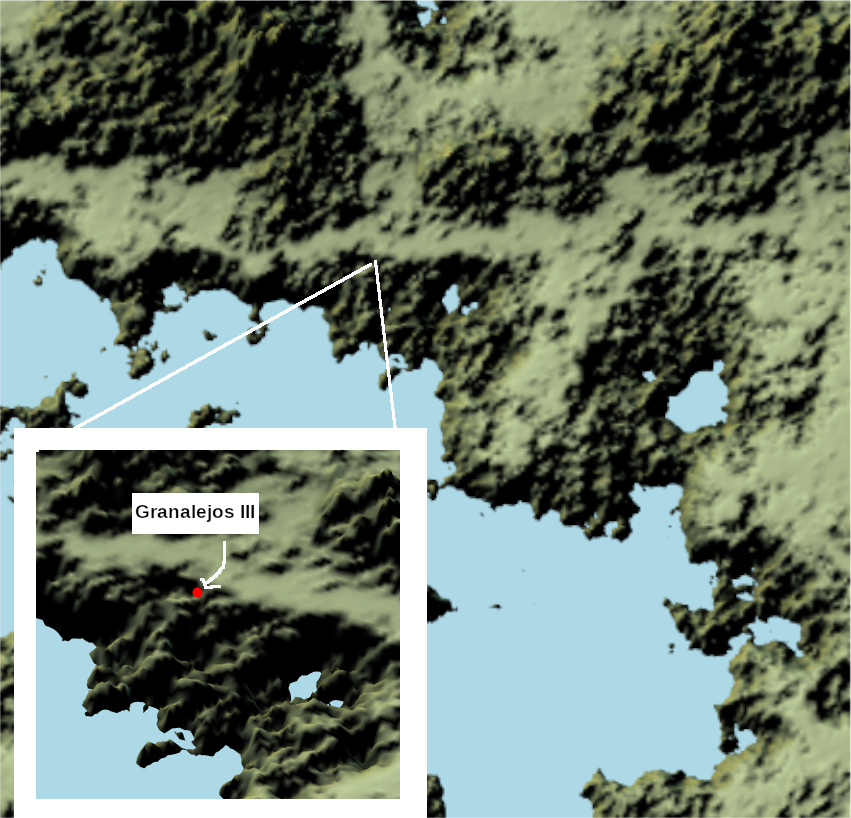
\includegraphics[width=.4\textwidth]{granalejors3}
                }
                \caption{New from Granalejos II}
            \end{figure}
        The engravings on ceramic artifacts were examined using a high-resolution 3D camera. The depictions were classified into different categories based on their subject matter, including battles, weapons, and violent acts. The frequency and distribution of these categories were then analyzed to determine the nature of the interactions between the Poppychewers and Rabbitskinners.
        \end{block}

        \column{.42\textwidth}
% Create the third block
        \begin{block}{\textbf{Analysis of the Engravings:}}
            

            The engravings on the ceramic artifact provide us with a unique glimpse into the relationship between the Poppychewers and the Rabbitskinners. From our analysis of the

            \begin{figure}
                \label{fig:twomaps}
                \centering
                \makebox[\textwidth][c]{
                    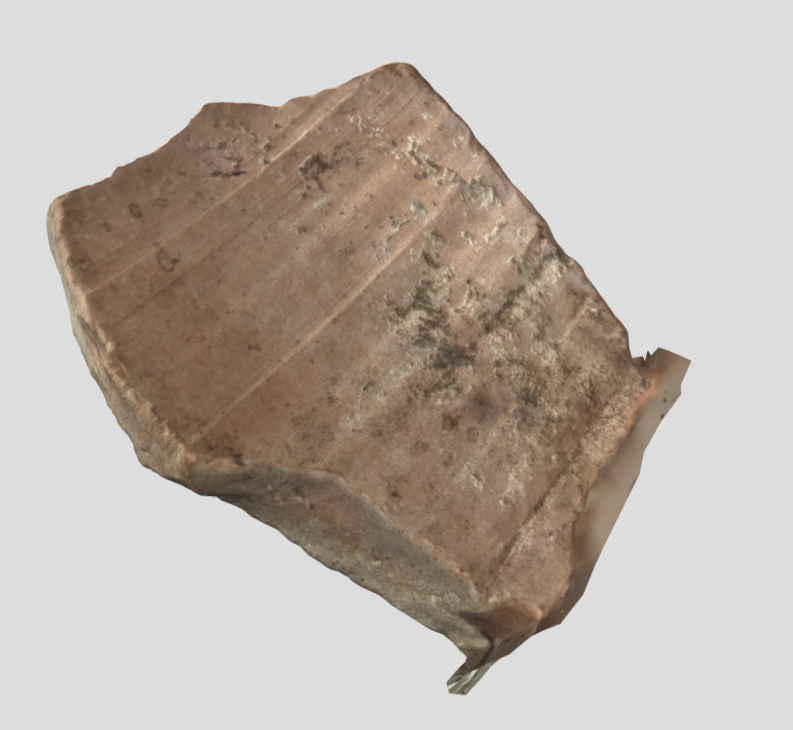
\includegraphics[width=.5\textwidth]{engrave}
                }
                \caption{New remains from Granalejos II}
            \end{figure}

        \end{block}

    \vfill
% Create the fourth block
    \begin{block}{\textbf{Conclusion}}
            The authors' TBE method provides a novel and powerful tool for studying the relationships between different populations in prehistoric times. The results of this study suggest that Rabbit-Skinners and Poppy-Chewers had a more symbiotic relationship characterized by trade and exchange rather than competition over resources. This study contributes to a better understanding of the history of Rabbithole and the nature of interactions between its inhabitants.
        \end{block}
        \column{.22\textwidth}

% Create the references block
        \begin{block}{\textbf{References}}
            Stone, H., \& Pants, F. (1966). Paleo-ecological reconstruction of rabbitholes environment. Journal of Ecological Research, 20(2), 45-56.
        \end{block}
        \vspace{8cm}
% Create the references block
    \begin{block}{\textbf{Additional note}}
        \small
    This project is part of the Archaoriddle project, funded by the British Academy - Leverhulme. If you want to help us understand what happened between Poppy-chewers and Rabbit-skinners flash the QR-code below. You will have a chance to receive a £650 grant to join us at the EAA in belfast! 
            \begin{figure}
                \includegraphics[width=.5\textwidth]{qrcode}
            \end{figure}
        \end{block}

    \end{columns}

\end{frame}
\end{document}



